\chapter{INTRODUCTION TO MACHINE LEARNING }\label{intro_to_ml}

\section{Machine Learning}

Machine learning is the modeling of complex systems on mathematical and statistical operations that perform tasks such as regression, classification and clustering using data. Thus, with the help of these algorithms computers can perceive mixed patterns in data. Today, there are many different machine learning methods for variety of data types. These learning methods are generally divided into three categories. These categories are supervised learning, unsupervised learning and reinforcement learning respectively. Supervised learning methods use training data with corresponding labels which defined beforehand. Label also known as ground truth represents the expected output of the machine learning system. This type of learning algorithms try to come up with a mapping function between training data and the ground truth. As an example, speech recognition \cite{speech_recognition} or a regression problem such as market forecasting \cite{market} can be solved using this type of learning. The second category is the methods implemented using only data without any corresponding ground truth. Two example of the areas of use of such unsupervised learning algorithms are the clustering problem in the recommender systems \cite{recommender_systems} and the dimension reduction \cite{pca}. The last category, reinforcement learning, is used in solving problems that require real-time decision making. For example, in the field of robotics, the methods under this category are used in the design of the systems to decide what action to take against any state in an environment \cite{robotics}.

Deep learning is a subclass of the much broader area of machine learning applications. In order to comprehend the methods mentioned in this thesis well, it is necessary to have a knowledge of statistics, calculus, optimization and computer vision as well as machine learning basics. For this reason, some machine learning basics are mentioned in the following chapters.

\section{Neural Networks}

The idea of a neural networks are although they could not be realized efficiently for a long time, is an idea in machine learning field that emerged more than 70 years ago, and represents a similarity to neurons in the human brain. First neural network is created by McCulloch an Pitts, however they did not have enough technology to run it. Later in 1954, Clark and Farley in MIT were able to run the first Neural Network.

The main feature that enables neural networks to work is that they are made of neurons. These neurons are similar to neurons in the human brain. The basic requirement for understanding how neural networks work is to understand how neurons in the human brain work and how it connects to Artificial Neural Networks (ANN).

There are billions of neurons in a human brain. These neurons communicate with each other using electrical signals. Neurons produce their own output according to the different types of signals they receive. If the value they receive is above a certain limit, it generates electrical impulse in response.

\begin{figure}[h]
    \centering
    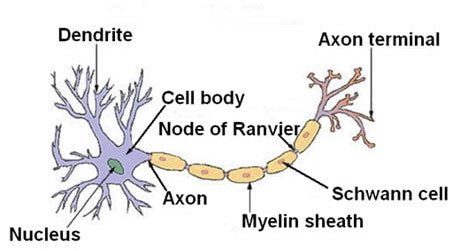
\includegraphics{figures/chapter3/braincell.png}
    \caption{Brain Neuron}
    \label{fig:brain_neuron}
\end{figure}

As with a real neuron, a neuron in the ANN also functions similarly. The neurons in the ANN simply take the input they receive and process this data and then give an output. Each neuron in the network has its own parameters called weights. This decision-making process produces an output yes or no. Hence, it is possible to call this process a classifier. Similar to a neuron function, a threshold function is illustrated in figure \ref{fig:threshold}.

\begin{figure}[h]
    \centering
    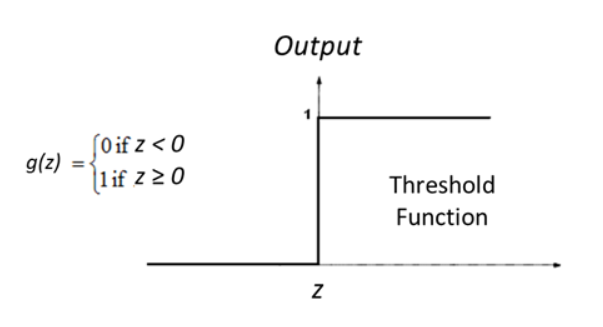
\includegraphics[scale=0.7]{figures/chapter3/threshol.png}
    \caption{Threshold Function}
    \label{fig:threshold}
\end{figure}

There are different numbers of layers in ANN depending on their size. Neurons transmit their output from each layer to the next layer. As will be explained later, the output from each neuron is inserted into activation functions to ensure non-linearity within the system. Neuron structure is shown in figure \ref{fig:neuron_drawl}.

\begin{figure}[h]
    \centering
    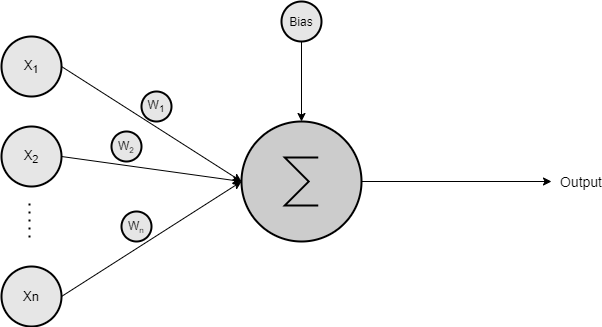
\includegraphics[scale=0.5]{figures/chapter3/neuron.png}
    \caption{Neuron}
    \label{fig:neuron_drawl}
\end{figure}

Based on the ideas previously announced, McCulloch and Pitts designed the first neural network. In the system they designed, many inputs are given to each neuron as input, and the output of the neuron can be obtained by adding these inputs after multiplying with weights. The output of this neuron is also directed to the activation function.Operations done in a neuron are shown in \ref{eqn:nn1} and \ref{eqn:nn2}.

\begin{equation}
\label{eqn:nn1}
    Out = \sum\limits_{i=1}^{N}{I_i W_i}
\end{equation}

\begin{equation}
\label{eqn:nn2}
    Y = f(Out)
\end{equation}

\subsection{Perceptron}

Mainly perceptron is a machine learning algorithm that classifies an input. Perceptron performs this classification with a linear function which uses weight and bias values. With this feature, perceptron forms the basis of all neural networks.

\begin{equation}
\label{eqn:perc}
    Out = \sum\limits_{i=1}^{N}{I_i W_i+B_i}
\end{equation}

Perceptron consists of 4 basic parts as input value, weight, bias and activation function. As can be seen, the innovation that perceptron adds to neural networks is that the bias value is added to each process as shown in \ref{eqn:perc}.

As was the case when neural networks were first launched, the perceptron could not achieve the expected success due to technical limitations. There are 2 types of Perceptron models which are called single-layered perceptron model and multi-layered perceptron model. It contains a feedforward network within the single-layer perceptron model. It is the simplest neural network that can be implemented. An illustration of a Feed-Forward network stucture is shown in \ref{fig:feed-forwardl}

\begin{figure}[h]
    \centering
    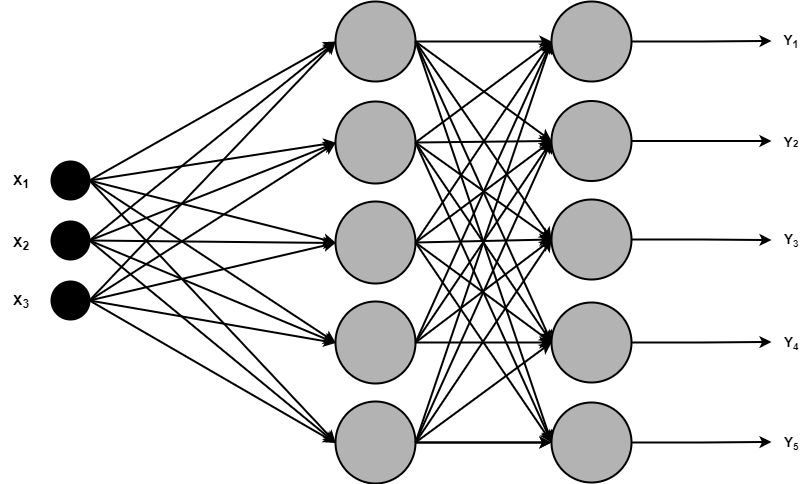
\includegraphics[scale=0.45]{figures/chapter3/FeedForward.png}
    \caption{Feed-Forward Network Structure}
    \label{fig:feed-forwardl}
\end{figure}

As seen in Figure \ref{fig:feed-forwardl}, each neuron in the first stage is connected to the neurons in the other layer. Combinations between all neurons require considerable high processing power which allow the solution of more complex problems. All neurons in the input layer direct their result to the output layer. If all the neurons between the layers are connected in a network, the network that is obtained can be called a fully connected network. On the other hand, if it is stated that the weight value between two different neurons, it is understood that there is no connection between that two neurons.

It is also pretty significant to state that single-layered perceptron models are only applicable to problems with linearly separable classes. Later on in the future, it is discovered that multi-layered perceptron networks can be used for non-linearly separable problems. Data distributions for different problems are given in figure \ref{fig:data-diff-dist}.

\begin{figure}[h]
    \centering
    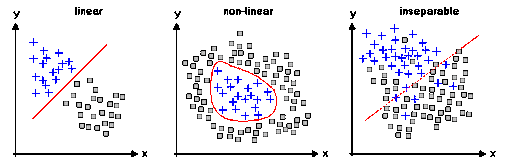
\includegraphics{figures/chapter3/linear-nonlinear-seperable.png}
    \caption{Data with Different Distributions}
    \label{fig:data-diff-dist}
\end{figure}

Even though multi-layered perceptron networks are similar to single-layered perceptron networks, they contain fundamental differences. There are many more hidden layers in multi-layered perceptron. Also, another important difference is that the multi-layer perceptron has a backward stage in addition to the forward stage.

In forward stage, a path from the input layer to the output layer is followed. In oppose to that in the backward stage, an error is obtained from the value from the generated output and the value that should actually be obtained, and this error is used to change the parameters in the neurons which are weights and biases.

One other important addition is the usage of non-linear activation functions in multi-layer networks. With these improvements, multi-layered networks are able to work on non-linearly separable problems.

\subsection{Loss Function}

In mathematics, loss function also known as cost function is a function that represents the real “cost” of anyting to a real value. In essence, optimization problems try to minimize the output of the loss functions. They are designed to take one or more values as input and return a real number as output. Mean square error (MSE) is a simple loss function commonly used in neural network models. It is the sum of squared distances between the predicted values and the corresponding ground truth values. An optimizer will update the neural network parameterswhile trying to minimize this loss. Cross entropy loss \cite{cross_entropy}, also known as log loss or logistic loss, mostly used in classification problems when the values of the output layer is either zero or one. For binary classification problems binary cross-entropy loss can be used. If there are more than two classes in the problem categorical cross-entropy loss is preferred. In equation \ref{eq:binary_cross_entropy} the binary cross-entropy formulation is presented where \(y\) is the binary indicator if label is correct classified or not and \(p\) is the predicted probability of that label. To sum up, loss function is a mathematical way of measuring the error between the prediction and ground truth in order to see how the model is performing.

\begin{equation}
    L = -(y \cdot log(p) + (1-y) \cdot log(1 - p))
    \label{eq:binary_cross_entropy}
\end{equation}

\subsection{Optimizer}

Algorithms that try to minimize the output of the loss function by changing the model parameters during the training phase are called optimizers. Optimizers are algorithms that calculate how and how much should the values of parameters updated. One of the most popular optimizer used in neural network applications is the Gradient Descent algorithm \cite{gradient_descent}. Simply put, this algorithm looks at the gradient of the loss value effect of a small change in network parameters. In computer vision studies, advanced optimizers such as Adam \cite{adam} used.

\subsection{Activation Function}

Activation function is a spesific function for calculating the output of a single neuron in the neural network. Problems which are linearly non-seperable can be solvable using non-linear activation functions such as sigmoid, hyperbolic tangent (tanh), and ReLU. In concolutional layers ReLU activation function is commonly used. The main advantage of this activation function is that while casting negative neuron output values to zero it allows a regularization in the network via not activating every neuron. These mentioned activation functions can be seen in figure \ref{fig:activation_functions}.

\begin{figure}[h]
    \centering
    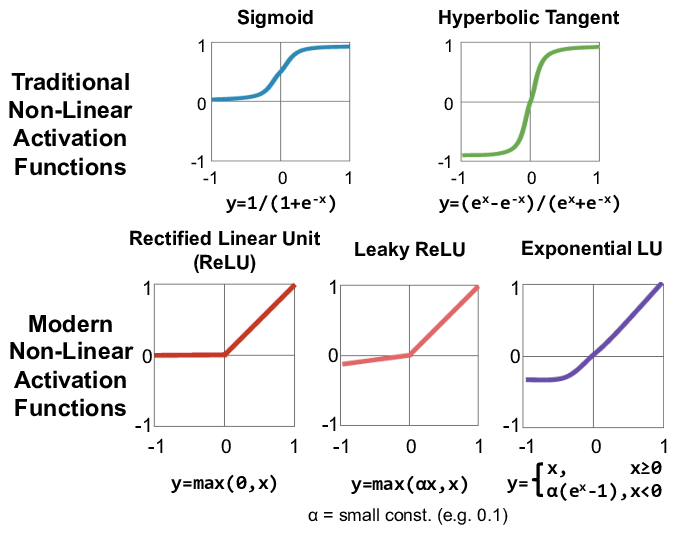
\includegraphics[width=10cm]{figures/chapter3/activation_functions.png}
    \caption{Activation Functions \cite{activation_functions}}
    \label{fig:activation_functions}
\end{figure}

\section{Convolutional Neural Networks}

Convolutional Neural Network is a widely used neural network architecture, especially thanks to its stunning success in computer vision studies \cite{leNet}. In this architecture, structures such as convolutional layer, pooling layer, flattening layer are used. CNNs are the structures that achieve only important features of the images by applying the convolution process using two-dimensional filters and obtaining different level of information in the image \cite{CNN_review}. CNN takes advantage of the hierarchical patterns in the data by following a path different than MLP structure. It brings together small and simple patterns to obtain more complex patterns. They use convolution operation in place of general matrix multiplication.

In the convolution layers, as seen in the figure \ref{fig:convolution}, 2D convolution is done between a tensor and the specified filter. In tasks such as inpainting where colored RGB images are used, these filters are applied separately to each color channel. During the convolution process while applying these filters which usually have 3x3, 5x5, or 7x7 size kernel onto matrix, on the borders padding process is applied. During this process, padding determines the course of action when values that are outside the limit and do not exist are desired to be accessed by convolution operation.

\begin{figure}[h]
    \centering
    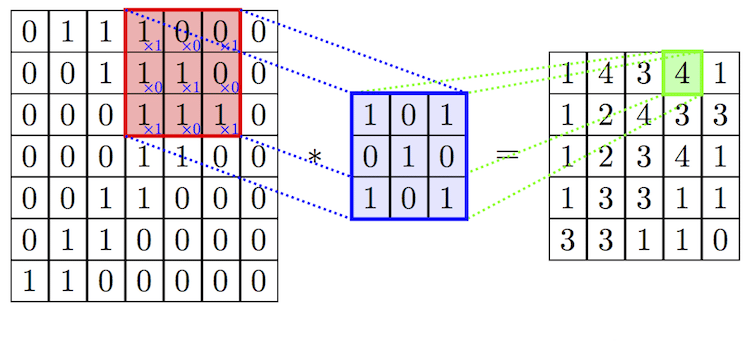
\includegraphics[width=10cm]{figures/chapter3/convolution.png}
    \caption{2D Convolution \cite{convolution_pooling}}
    \label{fig:convolution}
\end{figure}

Pooling layers, generally following the convolutional layers, reduce the size of the resulting tensor. In many convolutional neural networks, max pooling is used, but there are also min pooling and average pooling layers. The given tensor is divided into smaller pieces and a new and smaller tensor is obtained by taking the maximum, minimum or mean value of each sub-piece according to the chosen method. In figure \ref{fig:pooling}, average-pooling and max-pooling methods are shown.

\begin{figure}[h]
    \centering
    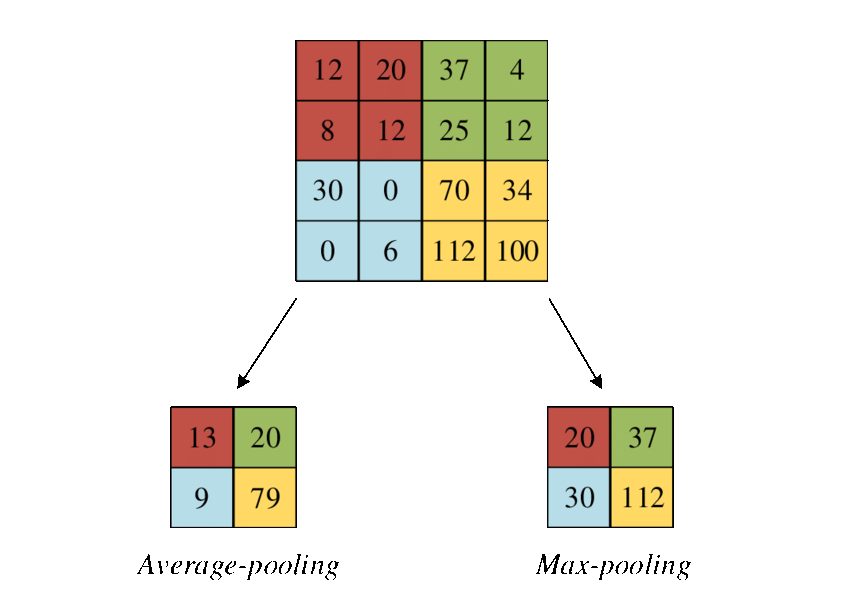
\includegraphics[width=10cm]{figures/chapter3/pooling.png}
    %\hspace{5cm} % gerekirse kullanabiliriz.
    \caption{Pooling \cite{convolution_pooling}}
    \label{fig:pooling}
\end{figure}

Flattening layer is the layer that makes the tensors in CNN structures vectorized in order to use the fully connected layers which commonly used in MLP structures. This layer serialized the incoming tensor and fills all the values to the neurons in a layer.

There are two CNN architectures commonly used for deep inpainting studies. First one is the encoder-decoder structures, and the other one is a derivation of the former one which called as autoencoder structure. These architectures performs well on many computer vision task and also shows promising results on other inverse problems in computer vision such as inpainting, denoising, and super-resolution. Moreover, this structures can work on different deep learning problems such as sentiment analysis, image captioning, and translation. For example, Google Translate is built upon an encoder-decoder structure \cite{google_translate}.

\subsection{Encoder-Decoder}

Enes yazacak.

\subsection{Autoencoder}

Enes yazacak.

\section{Generative Adversarial Networks}

As time passed, many different machine learning methods and ideas emerged. As explained in the neural network and machine learning sections, these methods were methods that work to make operations on the input to obtain meaning, or methods that uses datasets with huge amount of data with expected outputs to converge the model to give correct result.

As machine learning methods and specifically neural network and deep learning methods began to be used more frequently and the number of areas in which they were used increased, the methods used continued to differ and develop. One of these ideas developed is Generative Adversarial Networks.

It is possible to categorize methods of machine learning under 2 main categories, which are supervised and unsupervised learning. Even, it is possible to obtain successful results with supervised learning labeling huge amount of data is not economical and highly time consuming or in some cases it is not possible. Basically, the basic idea behind the emergence of the generative models is that there is no possible data that can be compared with output, or rather, the desired output does not have a correct answer to compare. Objectives of generator an discriminator models is given in figure \ref{fig:gan1}.

\begin{figure}[h]
    \centering
    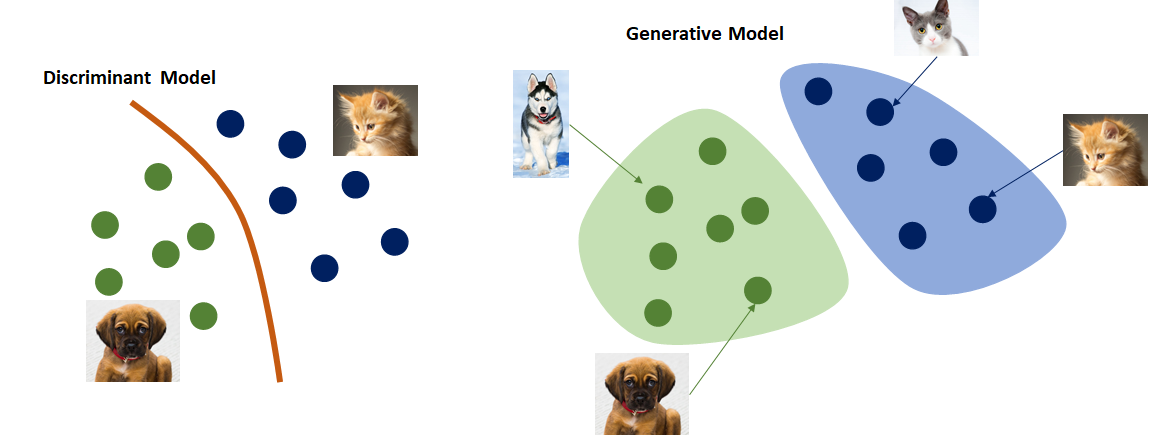
\includegraphics[scale=0.5]{figures/chapter3/generative-vs-discriminative-example.png}
    \caption{Difference Between Generative and Discriminative Models}
    \label{fig:gan1}
\end{figure}

There are different type of generative methods in machine learning. Most generative models developed over Markov chain and maximum likelihood estimation. Also, there are generative models such as Restricted Boltzmann Machine \cite{Boltzman} and Deep Belief Network \cite{deepbelief}.  A new model called Generative Adversarial Networks (GANs) is proposed by Ian Goodfellow \cite{gan} and it has been used in various problems in the area of computer vision.

\begin{figure}[h]
    \centering
    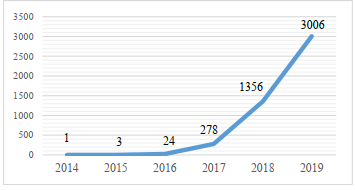
\includegraphics{figures/chapter3/gan-references-over-years.png}
    \caption{GAN Citation Counts}
    \label{fig:gancount}
\end{figure}

With the use and development of GANs in many different fields, GAN structures have become one of the leading methods of unsupervised learning. In figure \ref{fig:gancount}, work counts related to GAN is illustrated.

There are 2 different networks in the GAN. The word adversarial in its name comes from the fact that these structures work against each other throughout the training procedure.

As explained by Goodfellow \cite{gan}, within the GAN structure there are 2 networks being trained simultaneously. These networks are called generative and discriminative, respectively, G and D. In this structure, G is responsible for the creation of new data, while D tries to predict the probability of the data given as input to it.

From this point of view, it can be said that the Generative and Discriminator structures correspond to the minimax two-player game. Also, if G and D are constructed as perceptrons with multilayers, it can be said that the backpropagation can be used to train the whole structure. Simplified structure of GAN can be seen in figure \ref{fig:ganstruct}.

\begin{figure}[h]
    \centering
    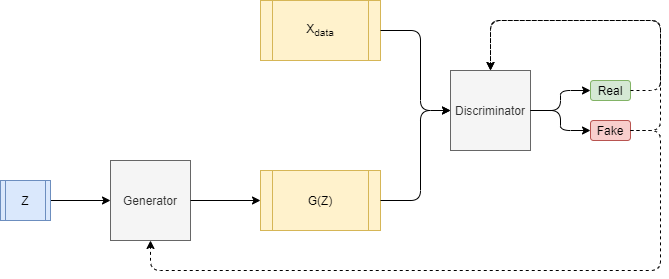
\includegraphics[scale=0.55]{figures/chapter3/GAN.png}
    \caption{GAN Model Explanation}
    \label{fig:ganstruct}
\end{figure}

When the mentioned adversarial model structure is implemented with perceptron, its application becomes straightforward. As a first step, generator structure G functions as a mapping to obtain data distribution from the input given to it. The discriminator structure created creates only a scalar as output. Structure D is trained to better label data from G and dataset. However, G is also trained to minimize log (1 - D (G (z))).

To explain, D and G play minimax with the function V (G, D) given in equation \ref{eqn:minmax}.

\begin{equation}
\label{eqn:minmax}
    min_Gmax_D V(D,G)= E_{x~P_{data(x)}}[logD(x)]+E_{z~P_{z}(Z)}[log(1-D(G(z)))]
\end{equation}

When implemented, it can be seen that Equation [] could not give sufficient results. As can be guessed, at the beginning of the training phase, the Discriminator structure generated data can be easily distinguished from the real data which causes log(1-D(G(Z)) to saturate. In this case, it is reasonable to train to minimize log(D(G(Z)) rather than train to minimize log(1-D(G(Z)).

\begin{figure}[h]
    \centering
    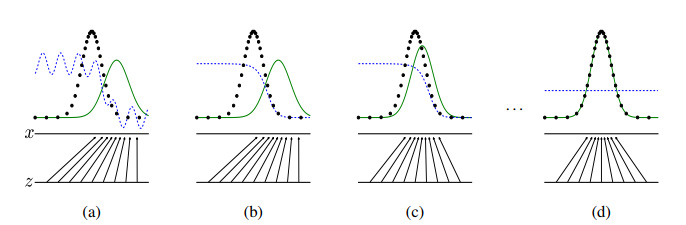
\includegraphics[scale=0.7]{figures/chapter3/gan-mapping.png}
    \caption{Mapping Effects}
    \label{fig:gan-mappingl}
\end{figure}

The bottom line shown in Figure \ref{fig:gan-mappingl}, represents the data, and the horizontal line above it shows the domain of the data generated. The upward arrows between these two lines also show how the x = G (z) mapping takes place. [Şurayı ANLAAAA VE ORIGINALDAN EKLE]

To exemplify the success of GAN structures, examples of faces produced by this method in different years are shown in Figure \ref{fig:gan-success}.

\begin{figure}[h]
    \centering
    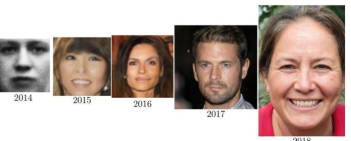
\includegraphics{figures/chapter3/gan-success-over-years.png}
    \caption{GAN Success Over Years}
    \label{fig:gan-success}
\end{figure}

\subsection{Deep Convolutional GAN}

Deep Convolutional Generative Adversarial Network \cite{dcgan}, shortly DCGAN, is a frequently used addition to GAN structures. The generator and discriminator used in this structure are in deep convolutional structure and thus a more stable training is performed. With this work, it is aimed to use the advantages of CNNs.

DCGAN is an important development in terms of having more successful and high quality generators. At the same time, this structure has helped the emergence of many different types of GAN structures. Overall stcuture of DCGAN is illustrated in figure \ref{fig:dcgan}.

\begin{figure}[h]
    \centering
    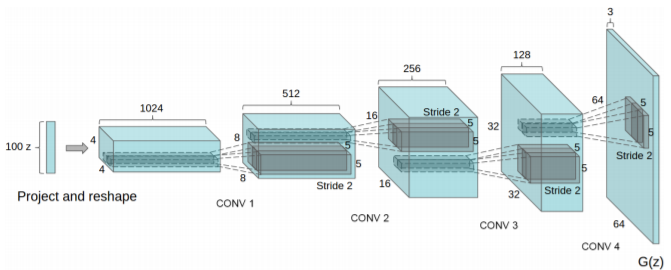
\includegraphics[scale=0.8]{figures/chapter3/dc-gan-structure.png}
    \caption{DCGAN Structure}
    \label{fig:dcgan}
\end{figure}

\subsection{Wasserstein GAN}

As GAN applications become widespread, different types of GAN structures have started to emerge. One of them is the Wasserstein GAN structure. This GAN structure both increases the stability of the GAN and provides the use of a loss function better related to the quality of the images produced.

WGAN model is a study presented by Arjovsky et al\cite{wgan}, that adds additional features to the GAN structure. As mentioned earlier, images in the WGAN structure, receive a score that expresses the reality of the image rather than simply being classified as real or fake by the discriminator.

Fundamentally plans to be a solution to Discriminator and Generator balancing, one of the main problems of GAN structures, with the new Earth Move distance using WGAN. Earth-Mover distance is shown in equation \ref{eqn:wgan}.

\begin{equation}
\label{eqn:wgan}
    W(P_r, P_g)= {inf}_{y\epsilon\prod (P_r,P_g)}\mathbb{E}_{(x,y)~y}[||x-y||]
\end{equation}
